\documentclass[12pt]{report}
\usepackage[utf8]{inputenc}
\usepackage[OT1]{fontenc} 
\usepackage{xspace}
\usepackage[frenchb]{babel}
\usepackage{times}
\usepackage{graphicx}
\usepackage[top=2in, bottom=1.5in, left=1in, right=1in]{geometry}

\graphicspath{{images/}}
\addtocounter{tocdepth}{3}
\setcounter{secnumdepth}{3}
\bibliographystyle{plain}
\renewcommand\thechapter {\Roman{chapter}}
 
\begin{document}

\newcommand\university{Université de Grenoble}
\newcommand\school{École doctorale EEATS}
\newcommand\structure{Laboratoire: Inria Grenoble Rhône-Alpes \\ Entreprise: Aldebaran}
\newcommand\auteur{Jory Lafaye}
\newcommand\encadrant{Dr. Pierre-Brice Wieber, Inria\\Dr. Cyrille Collette, Aldebaran\\Dr. Sebastien Dalibard, Aldebaran}
\newcommand\directeur{Dr. Bernard Brogliato, Inria\\~\\~}
\newcommand\titre{Commande des mouvements et de l'équilibre \\d'un robot humanoïde à roues omnidirectionnelles}

\begin{titlepage}

\newcommand{\HRule}{\rule{\linewidth}{0.5mm}} % Defines a new command for the horizontal lines, change thickness here

\center % Center everything on the page
 
%----------------------------------------------------------------------------------------
%	HEADING SECTIONS
%----------------------------------------------------------------------------------------

\textsc{\LARGE \university}\\[0.5cm] 
\textsc{\Large \school}\\[1.5cm] 
\textsc{\Large Thèse CIFRE}\\ 
\textsc{Présentée par}\\[0.5cm] 
\textsc{\Large \auteur}\\ [1.5cm] 
\textsc{\large \structure}\\[0.5cm] 

%----------------------------------------------------------------------------------------
%	TITLE SECTION
%----------------------------------------------------------------------------------------

\HRule \\[0.4cm]
{ \LARGE \bfseries \titre}\\[0.4cm] % Title of your document
\HRule \\[1.5cm]
 
%----------------------------------------------------------------------------------------
%	AUTHOR SECTION
%----------------------------------------------------------------------------------------

\begin{minipage}{0.4\textwidth}
\begin{flushleft} 
\emph{Directeur:}\\
\directeur
\end{flushleft}
\end{minipage}
~
\begin{minipage}{0.4\textwidth}
\begin{flushright} 
\emph{Encadrants:} \\
\encadrant
\end{flushright}
\end{minipage}\\[4cm]

% If you don't want a supervisor, uncomment the two lines below and remove the section above
%\Large \emph{Author:}\\
%John \textsc{Smith}\\[3cm] % Your name

%----------------------------------------------------------------------------------------
%	DATE SECTION
%----------------------------------------------------------------------------------------

%{\large Le \today}\\[3cm] % Date, change the \today to a set date if you want to be precise

%----------------------------------------------------------------------------------------
%	LOGO SECTION
%----------------------------------------------------------------------------------------

%\includegraphics{Logo}\\[1cm] % Include a department/university logo - this will require the graphicx package
 
%----------------------------------------------------------------------------------------

\vfill % Fill the rest of the page with whitespace

\end{titlepage}

\tableofcontents
\listoffigures

%
\newpage\cite{bib.miasa.2010}
%


\addcontentsline{toc}{chapter}{Résumé}

\chapter{Introduction}
	\section{Présentation de la plateforme expérimentale}
	\subsection{Pepper, un robot humanoïde à roues omnidirectionnelles}
	\subsection{Capteurs et actionneurs}
	\subsection{Propriétés mécaniques}	
\section{État de l'art}
	\subsection{Problématiques associées à Pepper}
	\subsection{Commande et équilibre des robots à roues}
		\subsubsection{Les robots à une et deux roues}
		\subsubsection{Les robots à trois roues et plus}
	\subsection{Commande et équilibre des robots bipèdes}
	\subsection{Synthèse et conclusion}
\section{Organisation du document}
	
\chapter{Modélisation et commande de Pepper}
	\chapter{Modélisation du système}
\section{Choix du modèle et conséquences}
	\subsection{Objectifs}
		L'objectif de ce chapitre est de présenter une modélisation dynamique d'un robot humanoïde possédant une base mobile à roues omnidirectionnelles. 
		Ce modèle doit apporter un bon compromis entre fidélité vis à vis du comportement du robot réel et complexité, qui impacte de manière directe le temps de calcul.
		Notamment, on montre qu'il n'est pas nécessaire de modéliser tout les paramètres du robot : représenter uniquement les dynamiques principales suffit à obtenir un contrôle précis du robot. 
		La section \ref{section.closedloop} détaillera les méthodes de compensation des éléments non modélisés.
	
		\fig{
			\centering
			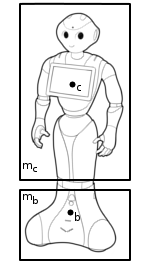
\includegraphics[width=2in]{modele.png}
			\caption{Représentation globale du modèle dynamique.}
			\label{fig.modele}
		}
		
	\subsection{Avantages du modèle}
		
		Le choix se porte sur une modélisation dynamique d'un robot rigide multi-corps. 
		Le modèle présenté \rfi{fig.modele} comporte deux corps. Le premier est attaché à la base mobile, de masse $m_b$ et de position du centre de masse (CoM) $\bar{b}$.
		Le second modélise l'ensemble du reste du robot, de masse $m_c$ et de CoM $\bar{c}$.
		
		Le choix d'un modèle à deux corps permet de prendre en compte la rotation générale du corps du robot autour de la base mobile.
		Cette modélisation est pertinente dans le cas où les bras du robot ne génèrent que peu ou pas de moment angulaire.
		Dans le cas contraire, nous considérerons que les effets parasites dû aux mouvements des bras pourront être compensés correctement par le schéma de contrôle en boucle fermée présenté en section \ref{section.closedloop}.
		Le choix de ce modèle est également conditionné par la répartition massique de la plate-forme expérimentale :
		Elle est principalement concentré en deux zones, qui correspondent aux corps choisis : la base mobile et le torse du robot.	
	
	\subsection{Inconvénients du modèle}
		
		Le choix d'un modèle rigide multi-corps implique que les éléments suivants ne seront pas modélisés :
		\liste{
			\item 	Les différentes élasticités. Les technologies d'actionnement utilisées sur la plate-forme expérimentale ne comportent pas d'élasticités notables.
				Le seul élément compliant est un ensemble de deux bandes élastiques attachées à l'articulation du roulis de la hanche permettant au robot de maintenir une posture droite en l'absence de contrôle du moteur.
				Cet élément est négligeable en terme de dynamique car la raideur associée est très faible.
			\item	Les jeux mécaniques présents sur le robot. Ceux-ci sont présents sur la plate-forme expérimentale, du fait de systèmes de réductions présents entre les moteurs et les articulations basés sur un système d'engrenages.
				Les effets dynamiques parasites apportés par le jeu mécanique ne sont pas négligeables.
				Cependant, il peuvent être compensés de manière suffisamment efficace (plus de détails en section \ref{section.closedloop}) pour que cela soit transparent du point de vue de la commande présentée dans le chapitre \ref{chapitre.commande}.
			\item	Les glissements pouvant survenir entre les roues du robot et le sols ne sont pas modélisés. 
				Ceux-ci peuvent être néanmoins handicapant, car le système devient en partie non-observable en présence de glissement (plus de détails en section \ref{section.observateurbase}).
				Une solution a été apportée en section \ref{section.objectifs3roues} afin de limiter leurs possibilités d'apparition ainsi que leurs impacts sur la dynamique du robot.
			\item	Le nombre de corps choisi pour cette modélisation dynamique est nécessairement plus faible que le nombre de corps réels présents sur le robot, pour des raisons de complexité du modèle.
				Ainsi, tout les effets dynamiques ne pourront pas être représentés. Le choix du nombre de corps, et de leurs propriétés doit permettre de rendre négligeable les dynamiques non modélisées.
				Le développement d'une solution optimale du choix du nombre de corps et de leurs propriété est présenté en annexe \ref{annexe.choixmodele}.
		}
		

	\section{Modélisation dynamique}

		\subsection{Problème de complémentarité mixte}
		
			\subsubsection{Géométrie du robot}
			
		
				On considère le robot modélisé par deux masses-point $\bar{b}$ et $\bar{c}$ de masse associée $m_b$ et $m_c$. 
				Ces corps sont en contact avec le sol par l'intermédiaire de trois points $p_f$, $p_r$ et $p_l$ correspondant aux trois points de contact des roues avec le sol \rfi{fig.bascule}.
				La roue avant gauche correspond au point $p_r$, la roue avant droite au point $p_l$ et la roue arrière au point $p_f$.
				On considère que le système peut être dans quatre mode dynamique différents :
				\liste{
					\item Le robot ne bascule pas et les trois roues sont en contact avec le sol.
					\item Le robot est en rotation vers l'avant autour de l'axe défini par les deux roues avant. On note l'angle de rotation $\psi_f$. La roue arrière est dans ce cas en l'air.
					\item Le robot est en rotation vers la gauche autour de l'axe défini par la roue avant gauche et la roue arrière. On note l'angle de rotation $\psi_l$. La roue avant droite est dans ce cas en l'air.
					\item Le robot est en rotation vers la droite autour de l'axe défini par la roue avant droite et la roue arrière. On note l'angle de rotation $\psi_r$. La roue avant gauche est dans ce cas en l'air.
				}
				Enfin, on la répartition de la masse de chaque corps est concentrée en un seul point. Ainsi, il n'y a aucune inertie de rotation associée à $\bar{b}$ ou $\bar{c}$
		
				\fig{
					\centering
					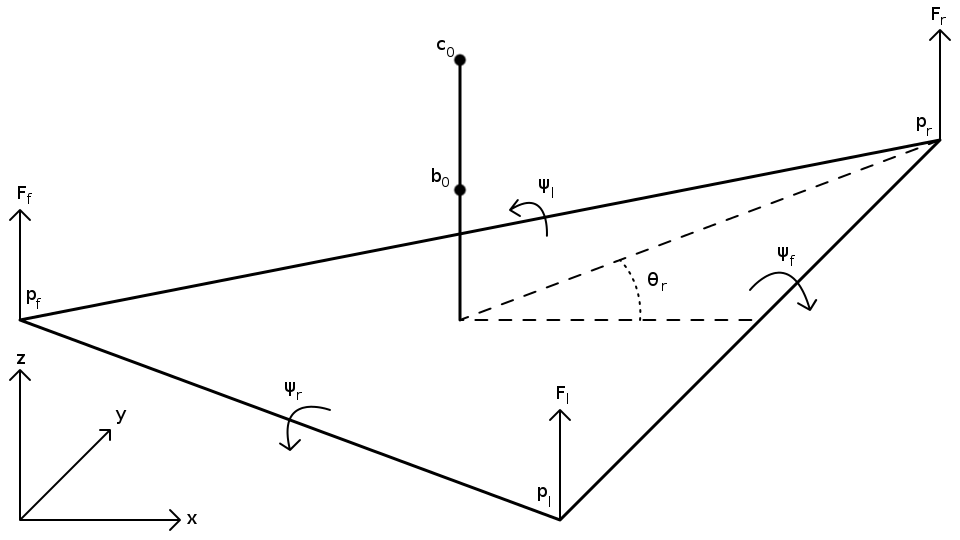
\includegraphics[width=6.5in]{bascule.png}
					\caption{représentation dans le repère $\rep_w$ des points de contacts avec le sol et des angles de basculement.}
					\label{fig.bascule}
				}
			\subsubsection{Cinématique directe}
			
				\subsubsubsection{Notations}
				
				
					Dans la suite, nous considèrerons un repère galiléen fixe orthonormé direct $\rep_w(O, \vec{x},\vec{y},\vec{z})$, $\vec{x}$ étant orienté vers l'avant du robot, $\vec{y}$ vers la gauche, et $\vec{z}$ vers le haut. 
					Ce repère est attaché au sol, $\vec{x}$ et $\vec{y}$ inclus dans le plan, et $\vec{z}$ orthogonal au sol. 
					Celui-ci n'est pas forcément horizontal, ce qui implique que le vecteur gravité ne soit pas forcément orienté selon l'axe $\vec{z}$.
					
					Premièrement, on considère que la position des corps $\bar{c}$ et $\bar{b}$ correspond à la composition de trois éléments \rfi{fig.lagrange}:
					\liste{
						\item $c_0$ et $b_0$ correspondent à la position d'origine de chaque corps par rapport à l'origine. Il est à noter que $c_0^{xy}=b_0^{xy}$.
						\item $\delta_c$ correspond à longueur apportée par l'actionnement des moteurs du robot. On peut noter du fait qu'il n'y a pas d'actionnement possible pour la base mobile, $\delta_b=0$.
						\item $\psi_f$, $\psi_r$ et $\psi_l$ correspondent aux rotations apportées par le basculement du robot sur chaqu'un de ses cotés.
					}
					
					Afin de pouvoir écrire les équations cinématiques, nous avons besoin de définir différentes grandeurs dépendantes de la géométrie du robot \rfi{fig.lagrange}\rfi{fig.bascule}. 
					
					\fig{
						\centering
						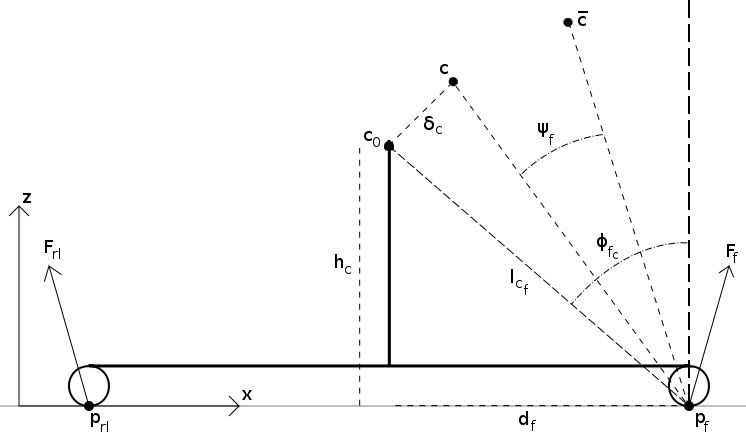
\includegraphics[width=6.5in]{lagrange.png}
						\caption{Projection dans le plan $(O,\vec{x}, \vec{z})$ du modèle du robot. 
							 Représentation des variables relatives au corps $\bar{c}$ et à l'angle $\psi_f$. 
							 Celles relatives à $\bar{b}$, $\psi_r$ et $\psi_l$ ne sont pas représentées, mais correspondent au même schéma.}
						\label{fig.lagrange}
					}
					$\forall i\in\{f,r,l\}$ :
					\liste{
						\item On note $\theta_i$ l'angle que fait le vecteur $\overrightarrow{b_0^{xy}~p_i^{xy}}$ avec l'axe $\vec{x}$. 
						On note $\vec{n_i}$ l'axe résultant et l'axe orthogonal $\vec{t_i}=\vec{z} \times \vec{n_i}$.
						$c_0$ et $b_0$ étant verticalement alignés, il en est de même pour le corps $\bar{c}$.
						On note $\rep_i$ le repère $(O, \vec{n}_i, \vec{t}_i, \vec{z})$.
						\item On note $\phi_{i_b}$ et $\phi_{i_c}$ les angles que font respectivement les vecteurs $\overrightarrow{b_0^{t_iz}~p_i^{t_iz}}$ et $\overrightarrow{c_0^{t_iz}~p_i^{t_iz}}$ avec l'axe $\vec{z}$.
						\item $l_{b_i}$ et $l_{c_i}$ correspondent aux normes des vecteurs $\overrightarrow{b_0^{xyz}~p_i^{xyz}}$ et $\overrightarrow{c_0^{xyz}~p_i^{xyz}}$.
						\item $d_i$ correspond à la norme du vecteur $\overrightarrow{b_0^{xy}~p_i^{xy}}$, qui est la même concernant le corps $\bar{c}$.
						\item $h_b$ et $h_c$ correspondent à la composante selon l'axe $\vec{z}$ des vecteurs $\overrightarrow{b_0^{xyz}~p_i^{xyz}}$ et $\overrightarrow{c_0^{xyz}~p_i^{xyz}}$.
					}
					
					
					Enfin, on note $b$ et $c$ les positions commandées des corps par rapport à l'origine $O$ :
					\eqa{
						b^{xyz} &= b_0^{xyz}\\
						c^{xy} &= c_0^{xy}+\delta_c^{xy}  = b_0^{xy} + \delta_c^{xy} \\
						c^z &= c_0^z + \delta_c^z = b_0^z + h_c + \delta_c^z
					}
					
				\subsubsubsection{Equations cinématiques}
					
					Nous pouvons à présent écrire les équations cinématiques des corps $\bar{c}$ et $\bar{b}$ :
					\eqa{
					\label{eq.cin_cx}
						\bar{c}^x &= c^x + \somme{i\in\{f, r, l\}}{}{d_i\cos(\theta_i) + l_{c_i}\sin(\phi_{i_c}+\psi_i)\cos(\theta_i)}  \\
					\label{eq.cin_cy}
						\bar{c}^y &= c^y + \somme{i\in\{f, r, l\}}{}{d_i\sin(\theta_i) + l_{c_i}\sin(\phi_{i_c}+\psi_i)\sin(\theta_i)} \\
					\label{eq.cin_cz}
						\bar{c}^z &= c^z + \somme{i\in\{f, r, l\}}{}{-h_c + l_{c_i}\cos(\phi_{i_c}+\psi_i)}
					}
					\eqa{
					\label{eq.cin_bx}
						\bar{b}^x &= b^x + \somme{i\in\{f, r, l\}}{}{d_i\cos(\theta_i) + l_{b_i}\sin(\phi_{i_b}+\psi_i)\cos(\theta_i)}  \\
					\label{eq.cin_by}
						\bar{b}^y &= b^y + \somme{i\in\{f, r, l\}}{}{d_i\sin(\theta_i) + l_{b_i}\sin(\phi_{i_b}+\psi_i)\sin(\theta_i)} \\
					\label{eq.cin_bz}
						\bar{b}^z &= b^z + \somme{i\in\{f, r, l\}}{}{-h_b + l_{b_i}\cos(\phi_{i_b}+\psi_i)}
					}
					
					Nous aurons besoin également des équations cinématiques des points $p_{frl}$. $\forall i\in\{f,r,l\}$ :
					
					\eqa{
					\label{eq.cin_px}
						p_{i}^{x} &= b^{x} + d_{i}\cos(\theta_{i}) + l_{b_{i}}\sin(\phi_{i_b}+\psi_{i})\cos(\theta_{i}) \\
					\label{eq.cin_pz}
						p_{i}^{x} &= b^{y} + d_{i}\sin(\theta_{i}) + l_{b_{i}}\sin(\phi_{i_b}+\psi_{i})\sin(\theta_{i}) \\
					\label{eq.cin_py}
						p_{i}^{z} &= b^{z} - h_b + l_{b_{i}}\cos(\phi_{i_b}+\psi_{i})
					}
				
				\subsubsubsection{Hypothèse d'angles de basculements faibles}
				
					Dans la suite, afin de simplifier les formulations des équations de la dynamique, nous allons établir dès maintenant une hypothèse : Les angles $\psi_{frb}$ sont considérés proches de $0$.
					Dans le cas où le robot ne bascule pas, cela est exact. Dans le cas où le robot bascule, on suppose le fait que l'angle de basculement reste faible.
					Nous pouvons donc réécrire les équations cinématiques \rf{eq.cin_cx}\rf{eq.cin_cy}\rf{eq.cin_cz}\rf{eq.cin_bx}\rf{eq.cin_by}\rf{eq.cin_bz} et \rf{eq.cin_px}\rf{eq.cin_py}\rf{eq.cin_pz} en utilisant une approximation du premier ordre :
					\eqa{
					\label{eq.cin_cx_appr}
						\bar{c}^x &= c^x + h_c\somme{i\in\{f, r, l\}}{}{\cos(\theta_i)\psi_i} \\
					\label{eq.cin_cy_appr}
						\bar{c}^y &= c^y + h_c\somme{i\in\{f, r, l\}}{}{\sin(\theta_i)\psi_i} \\
					\label{eq.cin_cz_appr}
						\bar{c}^z &= c^z + \somme{i\in\{f, r, l\}}{}{d_i\psi_i} \\
					\label{eq.cin_bx_appr}
						\bar{b}^x &= b^x + h_b\somme{i\in\{f, r, l\}}{}{\cos(\theta_i)\psi_i} \\
					\label{eq.cin_by_appr}
						\bar{b}^y &= b^y + h_b\somme{i\in\{f, r, l\}}{}{\sin(\theta_i)\psi_i} \\
					\label{eq.cin_bz_appr}
						\bar{b}^z &= b^z + \somme{i\in\{f, r, l\}}{}{d_i\psi_i}
					}

					\eqa{
					\label{eq.cin_px_appr}
						p_{frl}^{x} &= b^{x} - d_{frl}\cos(\theta_{frl}) \\
					\label{eq.cin_py_appr}
						p_{frl}^{y} &= b^{y} - d_{frl}\sin(\theta_{frl}) \\
					\label{eq.cin_pz_appr}
						p_{frl}^{z} &= b^{z} - h_b + 2d_{frl}\psi_{frl} 
					}
			
			\subsubsection{Énergies cinétiques et potentielles}
			
				\subsubsubsection{Contraintes sur le basculement du robot}
				\label{section.contrainte_basculement}
				
					Afin d'exprimer les équations du mouvement du robot, nous allons utiliser la méthode Lagrangienne.
					Celle-ci est pertinente dans notre cas car elle est particulièrement adaptée à la formulation sans ambiguïtés de systèmes dynamiques soumis à des forces de contraintes, comme les forces de réactions dues au sol sur les roues. 
					Pour cela, il nous faut dans un premier temps écrire les équations des énergies cinétiques $T$ et potentielles $V$ du système :
					
					\eqa{
						T &= \frac{1}{2}m_b(\dot{\bar{b}}^{x^2} + \dot{\bar{b}}^{y^2} + \dot{\bar{b}}^{z^2}) + \frac{1}{2}m_c(\dot{\bar{c}}^{x^2} + \dot{\bar{c}}^{y^2} + \dot{\bar{c}}^{z^2}) \\
						V &= m_bg^x\bar{b}^x + m_cg^x\bar{c}^x + m_bg^y\bar{b}^y + m_cg^y\bar{c}^y + m_bg^z\bar{b}^z + m_cg^z\bar{c}^z \\
					}
					avec $g$ le vecteur gravité. On rappelle que le repère $\rep_w$ étant attaché au sol, le vecteur gravité n'est pas forcément orienté selon la direction verticale $\vec{z}$, car le sol peut ne pas être horizontal.
					
					
					Nous allons considérer une autre hypothèse à partir de maintenant : Il ne peut pas y avoir plus d'un seul des angles $\psi_f$, $\psi_r$ et $\psi_l$ non-nul à la fois. 
					Cela correspond à supposer que le robot ne peut basculer que sur deux roues. On ne considère évidement pas le cas où le robot est en chute libre, ainsi que le cas où il ne bascule que sur une seule roue.
					On justifie cela par le fait que sa construction mécanique ne permet pas au robot de basculer sur une roue, sauf s'il subit une perturbation extrêmement forte.
					
					
					On obtient donc la contrainte suivante :
					\eq{
						\label{eq.contrainte_psi_ij}
						\forall (i,j)\in\{f, r, l\},~ i\neq j,~~ \psi_i\psi_j=0
					}
					
				\subsubsubsection{Formulation des énergies cinétiques et potentielles}
				
					En dérivant les équations cinématiques \rf{eq.cin_cx_appr}\rf{eq.cin_cy_appr}\rf{eq.cin_cz_appr}\rf{eq.cin_bx_appr}\rf{eq.cin_by_appr}\rf{eq.cin_bz_appr} et en utilisant la contrainte précédente \rf{eq.contrainte_psi_ij}, nous pouvons exprimer les vitesses des corps $\bar{c}$ et $\bar{b}$ élevés au carré.
					\eqa{
						\dot{\bar{c}}^{x^2} &= \dot{c}^{x^2} + h_c^2\somme{i\in\{f, r, l\}}{}{\cos(\theta_i)^2\dot{\psi}_i^2} + 2h_c\dot{c}^x\somme{i\in\{f, r, l\}}{}{\cos(\theta_i)\dot{\psi}_i} \\
						\dot{\bar{c}}^{y^2} &= \dot{c}^{y^2} + h_c^2\somme{i\in\{f, r, l\}}{}{\sin(\theta_i)^2\dot{\psi}_i^2} + 2h_c\dot{c}^y\somme{i\in\{f, r, l\}}{}{\sin(\theta_i)\dot{\psi}_i}\\
						\dot{\bar{c}}^{z^2} &= \dot{c}^{z^2} + \somme{i\in\{f, r, l\}}{}{d_i^2\dot{\psi}_i^2} + 2\dot{c}^{z}\somme{i\in\{f, r, l\}}{}{d_i\dot{\psi}_i} \\
						\dot{\bar{b}}^{x^2} &= \dot{b}^{x^2} + h_b^2\somme{i\in\{f, r, l\}}{}{\cos(\theta_i)^2\dot{\psi}_i^2} + 2h_b\dot{b}^x\somme{i\in\{f, r, l\}}{}{\cos(\theta_i)\dot{\psi}_i} \\
						\dot{\bar{b}}^{y^2} &= \dot{b}^{y^2} + h_b^2\somme{i\in\{f, r, l\}}{}{\sin(\theta_i)^2\dot{\psi}_i^2} + 2h_b\dot{b}^y\somme{i\in\{f, r, l\}}{}{\sin(\theta_i)\dot{\psi}_i}\\
						\dot{\bar{b}}^{z^2} &= \dot{b}^{z^2} + \somme{i\in\{f, r, l\}}{}{d_i^2\dot{\psi}_i^2} + 2\dot{b}^{z}\somme{i\in\{f, r, l\}}{}{d_i\dot{\psi}_i}
					}
			
				
					Voici donc la formulation des énergies cinétiques et potentielles en fonction des variables du système :
					
					\eqa{
						\nonumber T &= \frac{1}{2}m_b(\dot{b}^{x^2}+\dot{b}^{y^2}+\dot{b}^{z^2}) + \frac{1}{2}m_c(\dot{c}^{x^2}+\dot{c}^{y^2}+\dot{c}^{z^2}) + \frac{1}{2}(m_bh_b^2+m_ch_c^2)\somme{i\in\{f, r, l\}}{}{\dot{\psi}_i^2}\\
						\nonumber  &+ \frac{1}{2}(m_c+m_b)\somme{i\in\{f, r, l\}}{}{d_i^2\dot{\psi}_i^2}  + (m_ch_c\dot{c}^z+m_bh_b\dot{b}^z)\somme{i\in\{f, r, l\}}{}{d_i\dot{\psi}_i} \\
					\label{eq.T}
						&+ (m_bh_b\dot{b}^x+m_ch_c\dot{c}^x)\somme{i\in\{f, r, l\}}{}{\cos(\theta_i)\dot{\psi}_i} + (m_bh_b\dot{b}^y+m_ch_c\dot{c}^y)\somme{i\in\{f, r, l\}}{}{\sin(\theta_i)\dot{\psi}_i} \\
						\nonumber\\
						\nonumber V &= m_bg^xb^x + m_cg^xc^x + m_bg^yb^y + m_cg^yc^y + m_bg^zb^z + m_cg^zc^z \\
						\nonumber &+ (m_bg^x h_b + m_cg^x h_c)\somme{i\in\{f, r, l\}}{}{\cos(\theta_i)\psi_i} + (m_bg^y h_b + m_cg^y h_c)\somme{i\in\{f, r, l\}}{}{\sin(\theta_i)\psi_i} \\
					\label{eq.V}
						&+(m_b+m_c)g^z\somme{i\in\{f, r, l\}}{}{d_i\psi_i}
					}			
					
			
			\subsubsection{Coordonnées généralisées et Lagrangien}
			
				L'étape suivante dans la méthode Lagrangienne est d'exprimer l'équation du Lagrangien en fonction des coordonnées généralisées choisies.
				
				Habituellement, le choix des coordonnées généralisées correspondent aux degrés de libertés du système. 
				Afin de faciliter la formulation du modèle, nous allons plutôt utiliser le jeu de coordonnées $q$ suivant :
				\eq{
					q = \tr{\mat{b^x & b^y & b^z & c^x & c^y & c^z & \psi_f & \psi_r & \psi_l} }
				}
				
				Le choix d'utiliser les trois angles $\psi_{frl}$ pour représenter la rotation du système autour des trois directions possible permettra par la suite d'exprimer plus simplement les équations de la dynamique.
				
				Le Lagrangien $L$ du système est exprimé à partir des énergies cinétiques et potentielles de la façon suivante :
				\eq{
					L = T - V
				}
				
			\subsubsection{Application du principe de moindre action}	
			
				\subsubsubsection{Définitions}
				
					On défini l'action du système comme l'intégrale temporelle du Lagrangien. 
					Le principe de moindre action énonce que, dans le cas d'un système Lagrangien, l'action est stationnaire. Le plus souvent, cela correspond à un minimum, d'où le terme de ``moindre action''.
					
					Résoudre ce système emmène aux équations d'Euler-Lagrange, équivalentes du principe fondamental de la dynamique de Newton. 
					Dans le cas d'un système contraint par des forces de contact, on écrit :
					\eq{
					\label{eq.lagrange}
						\frac{d}{dt}\frac{\partial L}{\partial \dot{q}} + \frac{\partial L}{\partial q} = \somme{i\in\{f,r,l\}}{k\in\{x,y,z\}}{\frac{\partial p_{i}^k}{\partial q}F_{p_{i}}^k}
					}
					
					Afin de clarifier l'écriture des équations de la dynamique, on pose :
					\eqa{
						m_{hc} &= m_ch_c \\
						m_{hb} &= m_bh_b \\
						m_{q} &= m_{hc}h_c+m_{hb}h_b \\
						m_t &= m_c+m_b \\
						C_{\theta_i} &= \cos(\theta_i) \\
						S_{\theta_i} &= \sin(\theta_i)
					}
				
				\subsubsubsection{Équations de la dynamique}
				
					Les éléments de l'équation \rf{eq.lagrange} peuvent être calculés à l'aide des équations des énergies \rf{eq.T}\rf{eq.V} ainsi que des équations cinématiques \rf{eq.cin_px_appr}\rf{eq.cin_py_appr}\rf{eq.cin_pz_appr} :
					\eqa{
						\label{eq.T_lagrange}
						\frac{d}{dt}\frac{\partial L}{\partial \dot{q}} &=
						\mat{
							m_b\ddot{b}^x+m_bh_b\somme{i\in\{f, r, l\}}{}{\cos(\theta_i)\ddot{\psi}_i} \\
							m_b\ddot{b}^y+m_bh_b\somme{i\in\{f, r, l\}}{}{\sin(\theta_i)\ddot{\psi}_i} \\
							m_b\ddot{b}^z+m_bh_b\somme{i\in\{f, r, l\}}{}{d_i\ddot{\psi}_i} \\
							m_c\ddot{c}^x+m_ch_c\somme{i\in\{f, r, l\}}{}{\cos(\theta_i)\ddot{\psi}_i} \\
							m_c\ddot{c}^y+m_ch_c\somme{i\in\{f, r, l\}}{}{\sin(\theta_i)\ddot{\psi}_i} \\
							m_c\ddot{c}^z+m_ch_c\somme{i\in\{f, r, l\}}{}{d_i\ddot{\psi}_i} \\
							(m_q + m_td^2_f)\ddot{\psi}_f + m_{hb}(C_{\theta_f}\ddot{b}^x+S_{\theta_f}\ddot{b}^y-d_f\ddot{b}^z) + m_{hc}(C_{\theta_f}\ddot{c}^x+S_{\theta_f}\ddot{c}^y+d_f\ddot{c}^z) \\
							(m_q + m_td^2_r)\ddot{\psi}_r + m_{hb}(C_{\theta_r}\ddot{b}^x+S_{\theta_r}\ddot{b}^y-d_r\ddot{b}^z) + m_{hc}(C_{\theta_r}\ddot{c}^x+S_{\theta_r}\ddot{c}^y+d_r\ddot{c}^z) \\
							(m_q + m_td^2_l)\ddot{\psi}_l + m_{hb}(C_{\theta_l}\ddot{b}^x+S_{\theta_l}\ddot{b}^y-d_l\ddot{b}^z) + m_{hc}(C_{\theta_l}\ddot{c}^x+S_{\theta_l}\ddot{c}^y+d_l\ddot{c}^z)
						},
						\\
						\label{eq.V_lagrange}
						\frac{\partial L}{\partial q} &= \mat{
							m_bg^x \\
							m_bg^y \\
							m_bg^z \\
							m_cg^x \\
							m_cg^y \\
							m_cg^z \\
							(m_{hc} + m_{hb})\cos(\theta_f)g^x + (m_{hc} + m_{hb})\sin(\theta_f)g^y + m_td_fg^z \\
							(m_{hc} + m_{hb})\cos(\theta_r)g^x + (m_{hc} + m_{hb})\sin(\theta_r)g^y + m_td_rg^z \\
							(m_{hc} + m_{hb})\cos(\theta_l)g^x + (m_{hc} + m_{hb})\sin(\theta_l)g^y + m_td_lg^z
						},
					}
					\eq{
						\label{eq.P_lagrange}
						\frac{\partial p_{frl}^x}{\partial q} = \mat{
							1\\
							0 \\
							0 \\
							0 \\
							0 \\
							0 \\
							0 \\
							0 \\
							0 \\
						},
						\frac{\partial p_{frl}^y}{\partial q} = \mat{
							0\\
							1 \\
							0 \\
							0 \\
							0 \\
							0 \\
							0 \\
							0 \\
							0 \\
						},
						\frac{\partial p_f^z}{\partial q} = \mat{
							0 \\
							0 \\
							1 \\
							0 \\
							0 \\
							0 \\
							2d_f \\
							0 \\
							0 \\
						},
						\frac{\partial p_r^z}{\partial q} = \mat{
							0 \\
							0 \\
							1 \\
							0 \\
							0 \\
							0 \\
							0 \\
							2d_r \\
							0 \\
						},
						\frac{\partial p_l^z}{\partial q} = \mat{
							0 \\
							0 \\
							1 \\
							0 \\
							0 \\
							0 \\
							0 \\
							0 \\
							2d_l \\
						}
					}
					
				\subsubsubsection{Formulation standard}
				
					Les équations de la dynamique \rf{eq.lagrange} peuvent à présent être réécrites en utilisant la formulation standard utilisée en robotique :
					\eq{
					\label{eq.formulation_standard}
						M \ddot{q} - f(q) = \tr{J}(q)\lambda
					}
					où, en identifiant avec les équations \rf{eq.T_lagrange}\rf{eq.V_lagrange}\rf{eq.P_lagrange} :
					\eqa{
						\lambda &= \tr{\mat{F_{p_{l}}^x & F_{p_{r}}^x & F_{p_{b}}^x & F_{p_{l}}^y & F_{p_{r}}^y & F_{p_{b}}^y & F_{p_{l}}^z & F_{p_{l}}^z & F_{p_{b}}^z}}\\
						M&=\mat{
							M_{bc} & M_{c\psi} \\ 
							\tr{M}_{c\psi} & M_\psi
						}, 
						M_{\psi} = \mat{
							m_q+m_td_f^2 & 0 & 0 \\
							0 & m_q+m_td_r^2 & 0 \\
							0 & 0 & m_q+m_td_l^2 
						},
						\\
						M_{bc} &= \mat{
							m_b & 0 & 0 & 0 & 0 & 0 \\
							0 & m_b & 0 & 0 & 0 & 0 \\
							0 & 0 & m_b & 0 & 0 & 0 \\
							0 & 0 & 0 & m_c & 0 & 0 \\
							0 & 0 & 0 & 0 & m_c & 0 \\
							0 & 0 & 0 & 0 & 0 & m_c
						},
						M_{c\psi} = \mat{
							m_{hb}C_{\theta_f} & m_{hb}C_{\theta_r} & m_{hb}C_{\theta_l} \\
							m_{hb}S_{\theta_f} & m_{hb}S_{\theta_r} & m_{hb}S_{\theta_l} \\
							m_{hb}d_f & m_{hb}d_r & m_{hb}d_l \\
							m_{hc}C_{\theta_f} & m_{hc}C_{\theta_r} & m_{hc}C_{\theta_l} \\
							m_{hc}S_{\theta_f} & m_{hc}S_{\theta_r} & m_{hc}S_{\theta_l} \\
							m_{hc}d_f & m_{hc}d_r & m_{hc}d_l
						}, \\
					}
					\eqa{
						f(q) &= \mat{
							m_b g^x \\ 
							m_b g^y \\ 
							m_b g^z \\ 
							m_c g^x \\ 
							m_c g^y \\ 
							m_c g^z \\ 
							(m_{hc} + m_{hb})\cos(\theta_f)g^x + (m_{hc} + m_{hb})\sin(\theta_f)g^y + m_td_fg^z \\
							(m_{hc} + m_{hb})\cos(\theta_r)g^x + (m_{hc} + m_{hb})\sin(\theta_r)g^y + m_td_rg^z \\
							(m_{hc} + m_{hb})\cos(\theta_l)g^x + (m_{hc} + m_{hb})\sin(\theta_l)g^y + m_td_lg^z
						},\\
						\tr{J}(q) &= \mat{
							1 & 1 & 1 & 0 & 0 & 0 & 0 & 0 & 0 \\
							0 & 0 & 0 & 1 & 1 & 1 & 0 & 0 & 0 \\
							0 & 0 & 0 & 0 & 0 & 0 & 1 & 1 & 1 \\
							0 & 0 & 0 & 0 & 0 & 0 & 0 & 0 & 0 \\
							0 & 0 & 0 & 0 & 0 & 0 & 0 & 0 & 0 \\
							0 & 0 & 0 & 0 & 0 & 0 & 0 & 0 & 0 \\
							0 & 0 & 0 & 0 & 0 & 0 & 2d_f & 0 & 0 \\
							0 & 0 & 0 & 0 & 0 & 0 & 0 & 2d_r & 0 \\
							0 & 0 & 0 & 0 & 0 & 0 & 0 & 0 & 2d_l \\
						}
					}
					
			\subsubsection{Contraintes de complémentarité mixte}
			
				Afin de compléter la formulation de la dynamique, il reste maintenant à utiliser les \textit{a priori} que l'on dispose sur notre système et formuler les contraintes de complémentarité mixte.
				
				Dans un premier temps, le robot n'a pas la possibilité de pénétrer dans le sol, nous avons donc :
				\eq{
					\forall i\in\{f,r,l\}, \psi_i \geq 0
				}
				
				Aussi, lorsque que le robot bascule sur un des axes $\psi_{frl}$, la force résultante sur la roue opposée est nulle :
				\eq{
					\forall i\in\{f,r,l\}, (\psi_i > 0) \then F_i^{xyz} = 0
				}
				
				Ensuite, lorsque le robot est en contact avec le sol, les forces verticales sur les points de contacts sont nécessairement positives :
				\eq{
					\forall i\in\{f,r,l\}, F_i^z \geq 0
				}
				
				Enfin, nous avons défini en section \rf{section.contrainte_basculement} que le robot ne peut pas basculer sur plus d'un des trois axes à la fois :
				\eq{
					\forall (i, j) \in \{f,r,l\},~ i\neq j, ~~ \psi_i\psi_j = 0
				}
				
				Nous pouvons donc exprimer les contraintes de complémentarité mixte pour le système :
				\eq{
				\label{eq.contrainte_complementarite}
					\forall (i, j) \in \{f,r,l\},~ i\neq j, 
					\lst{
						0 \le \psi_i \perp \psi_j \ge 0 \\
						0 \le \psi_i \perp F_i^z \ge 0 \\
						\psi_i F_i^x = 0 \\
						\psi_i F_i^y = 0
					}
				}
				
			\subsubsection{Synthèse}
			
				Dans cette section, nous avons dans un premier temps défini les équations cinématiques associées au modèle du robot.
				Cela nous a permit d'établir une formulation Lagrangienne de la dynamique, puis de l'identifier à la formulation standard des systèmes mécaniques en robotique.
				Enfin, les \textit{a priori} que nous connaissons concernant le système dynamique nous ont permit d'établir des contraintes de complémentarité mixte sur celui-ci.
				
				
				
				Sans ces contraintes, il aurait été possible de résoudre analytiquement les équations temporelles du mouvement. Cependant, la présence de celles-ci imposent une résolution particulière.
				Une première approche, qui sera développée dans les sections suivantes, est d'énoncer d'autres \textit{a priori} afin de fixer le problème de complémentarité
				(par exemple, en considérant que le robot n'est pas en possibilité de basculer, ou est en état de basculement sur un axe). 
				
				Ces approches ne permettent cependant pas de résoudre le problème complet. 
				Nous détaillerons dans la section \rf{section.modelisation_unifiee} une méthode de résolution du système complet \rf{eq.formulation_standard}\rf{eq.contrainte_complementarite}.
		
		\subsection{Cas où les trois roues sont en contact avec le sol}
			
			\subsubsection{Modèle dynamique}
				
				Lorsque le robot est en situation nominale, ses trois roues sont en contact avec le sol. 
				Les mouvements contrôlés du robot ne doivent également pas le faire basculer sur deux roues.
				Il est donc pertinent de modéliser le système dynamique dans le cas où les trois roues sont en contact avec le sol, 
				car en l'absence de forte perturbations, le contrôleur développé en section \rf{section.mpc_trois_roues} assure cette hypothèse.
			
				Définir le fait que le robot est en contact avec le sol avec ces trois roues permet de résoudre le problème de complémentarité de la façon suivante :
				\eq{
					\psi_{f} = \psi_{r} = \psi_{l} = 0
				}
				
				Ainsi, le jeu de variables $q$ devient :
				\eq{
					q = \tr{\mat{b^x & b^y & b^z & c^x & c^y & c^z}}
				}
				et l'on peut écrire le modèle dynamique correspondant :
				\eq{
				\label{eq.modele_trois_roues}
					M \ddot{q} - f(q) = \tr{J}(q)\lambda
				}
				avec :			
				\eqa{
					q_i &= \tr{\mat{b^x & b^y & b^z & c^x & c^y & c^z}} \\
					\lambda &= \tr{\mat{F_{p_{l}}^x & F_{p_{r}}^x & F_{p_{b}}^x & F_{p_{l}}^y & F_{p_{r}}^y & F_{p_{b}}^y & F_{p_{l}}^z & F_{p_{l}}^z & F_{p_{b}}^z}}\\
				\label{eq.force_contrainte_trois_roues}
					F_{p_{f}}^z &\ge 0,~~ F_{p_{r}}^z \ge 0,~~ F_{p_{l}}^z \ge 0 \\
					M &= \mat{
						m_b & 0 & 0 & 0 & 0 & 0 \\
						0 & m_b & 0 & 0 & 0 & 0 \\
						0 & 0 & m_b & 0 & 0 & 0 \\
						0 & 0 & 0 & m_c & 0 & 0 \\
						0 & 0 & 0 & 0 & m_c & 0 \\
						0 & 0 & 0 & 0 & 0 & m_c
					},
				}
				\eqa{
					f(q) &= \mat{
						m_b g^x \\ 
						m_b g^y \\ 
						m_b g^z \\ 
						m_c g^x \\ 
						m_c g^y \\ 
						m_c g^z 
					},
					\tr{J}(q) = \mat{
						1 & 1 & 1 & 0 & 0 & 0 & 0 & 0 & 0 \\
						0 & 0 & 0 & 1 & 1 & 1 & 0 & 0 & 0 \\
						0 & 0 & 0 & 0 & 0 & 0 & 1 & 1 & 1 \\
						0 & 0 & 0 & 0 & 0 & 0 & 0 & 0 & 0 \\
						0 & 0 & 0 & 0 & 0 & 0 & 0 & 0 & 0 \\
						0 & 0 & 0 & 0 & 0 & 0 & 0 & 0 & 0 
					}
				}
			
			\subsubsection{Définition du Centre de Pression}
			
				Dans le cas d'un système dont les positions des forces de contact sont définis sur un plan, il est possible de définir une grandeur nommé Centre de Pression $d^{xy}$ (CoP).
				Le CoP correspond au point dans le plan où le moment angulaire de la résultante des forces de contact est nul.
				La propriété essentielle du CoP est que celui est toujours défini à l'intérieur du polygone de l'enveloppe convexe définie par la position des forces de contact.
				Cela est dû aux contraintes de non-pénétration dans le sol des forces de contact \rf{eq.force_contrainte_trois_roues}.
				Lorsque le CoP est strictement à l'intérieur de ce polygone de support, le robot ne peut pas basculer sur deux roues.
				
				Ainsi, l'utilisation du CoP permet de manipuler de façon pertinente la somme des forces de contact afin de permettre au robot de ne jamais basculer de lui-même.
				Son expression est la suivante :
				\eq{
					d^{xy} = \frac{\somme{i\in\{f,r,l\}}{}{(p \times F)^{xy}}}{\somme{i\in\{f,r,l\}}{}{F_i^z}}
				}
				
			
			\subsubsection{Principe du moment angulaire}
			
				Le modèle de notre robot n'est pas un système fermé. Il n'y a donc pas de conservation du moment angulaire intrinsèque : Le lagrangien n'est pas invariant par rotation.
				Cependant, notre système est soumis à deux types de forces différentes : La première est due à la gravité, et dérive donc d'un potentiel, les secondes sont dues à des efforts de contacts, qui sont des contraintes concernant le sstème.
				Il est possible d'exprimer le principe du moment angulaire dans ce cas là, celui-ci se formule alors :
				
				\eq{
					q \times \prt{\dfrac{d}{dt}\dfrac{\partial L}{\partial \dot{q}} - \dfrac{\partial L}{\partial q}}  = \somme{i\in\{f,r,l\}}{}{p_i \times F}
				}
				
				En utilisant l'équation du modèle dynamique \rf{eq.modele_trois_roues}, on peut donc écrire le principe du moment angulaire autour des axes $\vec{y}$ et $\vec{x}$ :
				\eqa{
				\label{eq.moment_y_trois_roues}
					m_b(\ddot{b}^z-g^z)b^x -m_b(\ddot{b}^x-g^x)b^z + m_c(\ddot{c}^z-g^z)c^x - m_c(\ddot{c}^x-g^x)c^z &= \somme{i\in\{f,r,l\}}{}{p_i^xF_i^z-p_i^zF_i^x} \\
				\label{eq.moment_x_trois_roues}
					m_b(\ddot{b}^z-g^z)b^y -m_b(\ddot{b}^y-g^y)b^z + m_c(\ddot{c}^z-g^z)c^y - m_c(\ddot{c}^y-g^y)c^z &= \somme{i\in\{f,r,l\}}{}{p_i^yF_i^z-p_i^zF_i^y}
				}
				
			\subsubsection{Formulation du Centre de Pression et simplifications}
			
				On rappelle les équations du mouvement sur l'axe $\vec{z}$ \rf{eq.modele_trois_roues} :
				\eq{
				\label{eq.dyn_z_trois_roues}
					m_b(\ddot{b}^z-g^z) + m_c(\ddot{c}^z-g^z) = \somme{i\in\{f,r,l\}}{}{F_i^z}
				}
			
				En utilisant les équations résultantes du principe du moment angulaire autour des axes $\vec{y}$ et $\vec{x}$ \rf{eq.moment_y_trois_roues}\rf{eq.moment_x_trois_roues} ainsi que l'équation \rf{eq.dyn_z_trois_roues}, on peut formuler le CoP de la façon suivante :	
				\eq{
				\label{eq.cop_trois_roues}
					d^{xy} = \frac{m_b(\ddot{b}^z-g^z)b^{xy} -m_b(\ddot{b}^{xy}-g^{xy})b^z + m_c(\ddot{c}^z-g^z)c^{xy} - m_c(\ddot{c}^{xy}-g^{xy})c^z}  {m_b(\ddot{b}^z-g^z) + m_c(\ddot{c}^z-g^z)} \\
				}
				
				Notre objectif va être maintenant de linéariser l'équation \rf{eq.cop_trois_roues} par rapport aux variables commandées $c^{xy}$ et $b^{xy}$.
				Cela va nous permettre d'utiliser un contrôleur basé sur un système linéaire, ce qui est généralement beaucoup plus efficace en terme de temps de calcul qu'un contrôleur basé sur un système non-linéaire.
				
				On peut dans un premier temps noter que $b^z$ est constant à la hauteur $h_b$, car $b=b_0$. Ensuite, on contraint $c^z$ à être constant à la hauteur $h_c$.
				Enfin, on considère la gravité orientée selon l'axe $\vec{z}$ : $g=\tr{\mat{0, 0, -g_n}}$, avec $g_n = \norm{g}$, ce qui correspond à un sol horizontal.
				
				En utilisant ces \textit{a priori}, l'équation de la dynamique \rf{eq.cop_trois_roues} se réécrit :
				
				\eq{
					d^{xy} = \frac{m_bgb^{xy} -m_b\ddot{b}^{xy}h_b + m_cgc^{xy} - m_c\ddot{c}^{xy}h_c}  {(m_b + m_c)g} 
				}
				
				Enfin, les trois contraintes \rf{eq.force_contrainte_trois_roues} impliquent que $d^{xy}$ est à l'intérieur du triangle défini par les trois points de contacts :
				\eqa{
					d^{xy} \times (p_r^{xy}-p_f^{xy}) &\ge 0 \\
					d^{xy} \times (p_l^{xy}-p_r^{xy}) &\ge 0 \\
					d^{xy} \times (p_f^{xy}-p_l^{xy}) &\ge 0
				}
			
			\newpage
			~
			\newpage
			

		
		\subsection{Le robot bascule sur deux roues}

			On résout la complémentarité :
			\eq{
				\forall (i,j,k)\in\{f,r,l\}, i\neq j\neq k,~ \psi_{jk} = 0, F_i^{xyz} = 0
			}
			
			Le modèle dynamique devient :
			\eq{
				M \ddot{q} - f(q) = \tr{J}(q)\lambda
			}
			
			En identifiant :
			\eqa{
				q_i &= \tr{\mat{b^x & b^y & b^z & c^x & c^y & c^z & \psi_i}} \\
				\lambda &= \tr{\mat{F_{p_{j}}^x & F_{p_{k}}^x & F_{p_{j}}^y & F_{p_{k}}^y & F_{p_{j}}^z & F_{p_{k}}^z}}\\
				M &= \mat{
					m_b & 0 & 0 & 0 & 0 & 0 & m_{hb}C_{\theta_i} \\
					0 & m_b & 0 & 0 & 0 & 0 & m_{hb}S_{\theta_i} \\
					0 & 0 & m_b & 0 & 0 & 0 & m_{hb}d_i \\
					0 & 0 & 0 & m_c & 0 & 0 & m_{hc}C_{\theta_i} \\
					0 & 0 & 0 & 0 & m_c & 0 & m_{hc}S_{\theta_i} \\
					0 & 0 & 0 & 0 & 0 & m_c & m_{hc}d_i \\
					m_{hb}C_{\theta_i} & m_{hb}S_{\theta_i} & m_{hb}d_i & m_{hc}C_{\theta_i} & m_{hc}S_{\theta_i} & m_{hc}d_i & m_q+m_td_i^2
				},\\
				f(q) &= \mat{
					m_b g^x \\ 
					m_b g^y \\ 
					m_b g^z \\ 
					m_c g^x \\ 
					m_c g^y \\ 
					m_c g^z \\ 
					(m_{hc} + m_{hb})\cos(\theta_i)g^x + (m_{hc} + m_{hb})\sin(\theta_i)g^y + m_td_ig^z \\
				},\\
				\tr{J}(q) &= \mat{
					1 & 1 & 0 & 0 & 0 & 0 \\
					0 & 0 & 1 & 1 & 0 & 0 \\
					0 & 0 & 0 & 0 & 1 & 1 \\
					0 & 0 & 0 & 0 & 0 & 0 \\
					0 & 0 & 0 & 0 & 0 & 0 \\
					0 & 0 & 0 & 0 & 0 & 0 \\
					0 & 0 & 0 & 0 & 2d_j & 0 \\
					0 & 0 & 0 & 0 & 0 & 2d_k \\
				}
			}
			
			Principe du moment angulaire autour de l'axe $y$ et $x$ :
			\eqa{
				 \nonumber&m_b(\ddot{b}^z-g^z)b^x + m_bh_bd_i\ddot\psi_i\prt{b^x+h_b\cos(\theta_i)\psi_i} -m_b(\ddot{b}^x-g^x)b^z - m_bh_b\cos(\theta_i)\ddot\psi_ib^z\\
				 \nonumber+&m_c(\ddot{c}^z-g^z)c^x + m_ch_cd_i\ddot\psi_i\prt{c^x+h_c\cos(\theta_i)\psi_i} - m_c(\ddot{c}^x-g^x)c^z - m_ch_c\cos(\theta_i)\ddot\psi_ic^z\\
				 =& \somme{s\in\{j,k\}}{}{p_s^xF_s^z-p_s^zF_s^x}
			}
			\eqa{
				 \nonumber&m_b(\ddot{b}^z-g^z)b^y + m_bh_bd_i\ddot\psi_i\prt{b^y+h_b\sin(\theta_i)\psi_i} -m_b(\ddot{b}^y-g^y)b^z - m_bh_b\sin(\theta_i)\ddot\psi_ib^z\\
				 \nonumber+&m_c(\ddot{c}^z-g^z)c^y + m_ch_cd_i\ddot\psi_i\prt{c^y+h_b\sin(\theta_i)\psi_i} - m_c(\ddot{c}^y-g^y)c^z - m_ch_c\sin(\theta_i)\ddot\psi_ic^z\\
				 =& \somme{s\in\{j,k\}}{}{p_s^yF_s^z-p_s^zF_s^y}
			}
			
			Equation du mouvement sur l'axe $z$ :
			\eq{
				m_b(\ddot{b}^z-g^z) + m_bh_bd_i\ddot\psi_i + m_c(\ddot{c}^z-g^z) + m_ch_cd_i\ddot\psi_i = \somme{s\in\{j,k\}}{}{F_s^z}
			}
			
			Equation du CoP $d^{xy}$ :
			
			\eq{
				d^{xy} = \frac{\somme{i\in\{f,r,l\}}{}{p^{xy} \times F^{xy}}}{\somme{i\in\{f,r,l\}}{}{F_i^z}}
			}
			
			\eqa{
				\nonumber d^x &= \frac{m_b\prt{\ddot{b}^z-g^z+h_bd_i\ddot\psi_i}\prt{b^x+h_b\cos(\theta_i)\psi_i} - m_b\prt{\ddot{b}^x-g^x + h_b\cos(\theta_i)\ddot\psi_i}b^z}
				           {m_b(\ddot{b}^z-g^z) + m_c(\ddot{c}^z-g^z) + (m_bh_b+m_ch_c)d_i\ddot\psi_i} \\
				    &+ \frac{m_c\prt{\ddot{c}^z-g^z+h_cd_i\ddot\psi_i}\prt{c^x+h_c\cos(\theta_i)\psi_i} - m_c\prt{\ddot{c}^x-g^x + h_c\cos(\theta_i)\ddot\psi_i}c^z}
				           {m_b(\ddot{b}^z-g^z) + m_c(\ddot{c}^z-g^z) + (m_bh_b+m_ch_c)d_i\ddot\psi_i}
			}
			\eqa{
				\nonumber d^y &= \frac{m_b\prt{\ddot{b}^z-g^z+h_bd_i\ddot\psi_i}\prt{b^y+h_b\sin(\theta_i)\psi_i} - m_b\prt{\ddot{b}^y-g^y + h_b\sin(\theta_i)\ddot\psi_i}b^z}
				           {m_b(\ddot{b}^z-g^z) + m_c(\ddot{c}^z-g^z) + (m_bh_b+m_ch_c)d_i\ddot\psi_i} \\
				    &+ \frac{m_c\prt{\ddot{c}^z-g^z+h_cd_i\ddot\psi_i}\prt{c^y+h_b\sin(\theta_i)\psi_i} - m_c\prt{\ddot{c}^y-g^y + h_c\sin(\theta_i)\ddot\psi_i}c^z}
				           {m_b(\ddot{b}^z-g^z) + m_c(\ddot{c}^z-g^z) + (m_bh_b+m_ch_c)d_i\ddot\psi_i}
			}

			Les variables contrôlées sont directement $c^{xy}, b^{xy}$. $b^z$ est constant à la hauteur $h_b$ et on contraint $c^z$ à être constant à la hauteur $h_c$.
			De plus, la gravité est considérée selon l'axe z : $g=\tr{\mat{0, 0, -g}}$. Enfin, on considère $d_i=0$, ce qui correspond à négliger $d_i$ devant $h_b$ et $h_c$.
			
			\eqa{
				\nonumber d^x &= \frac{m_bg\prt{b^x+h_b\cos(\theta_i)\psi_i} + m_cg\prt{c^x+h_c\cos(\theta_i)\psi_i}}{(m_b+m_c)g} \\
				    &- \frac{m_bh_b\prt{\ddot{b}^x + h_b\cos(\theta_i)\ddot\psi_i}- m_ch_c\prt{\ddot{c}^x + h_c\cos(\theta_i)\ddot\psi_i}}{(m_b+m_c)g}
			}
			\eqa{
				\nonumber d^y &= \frac{m_bg\prt{b^y+h_b\sin(\theta_i)\psi_i} + m_cg\prt{c^y+h_c\sin(\theta_i)\psi_i}}{(m_b+m_c)g} \\
				    &- \frac{m_bh_b\prt{\ddot{b}^y + h_b\sin(\theta_i)\ddot\psi_i}- m_ch_c\prt{\ddot{c}^y + h_c\sin(\theta_i)\ddot\psi_i}}{(m_b+m_c)g}
			}
			
			Les deux contraintes $ F^z_{jk} \ge 0$ impliquent que $d^{xy}$ est dans le segment défini par les deux points de contact. 
			Pour assurer le maximum de robustesse, on choisi de contraindre le CoP au centre du segment :
			\eqa{
				d^x &= b^x + d_i\cos(\theta_i) \\
				d^y &= b^y + d_i\sin(\theta_i) 
			}
			
			On peut donc réécrire les équations précédente pour faire apparaitre la dynamique de $\psi_i$ par rapport à celles de $b$ et $c$ :
			\eqa{
				\label{eq.model_psi_x}
				\nonumber &(m_bh_b+m_ch_c)g\cos(\theta_i)\psi_i - (m_bh_b^2+m_ch_c^2)\cos(\theta_i)\ddot\psi_i \\
				=&~m_bh_b\ddot{b}^x + m_ch_c\ddot{c}^x - m_cg(c^x-b^x) - (m_c+m_b)gd_i\cos(\theta_i)
			}
			\eqa{
				\label{eq.model_psi_y}
				\nonumber &(m_bh_b+m_ch_c)g\sin(\theta_i)\psi_i - (m_bh_b^2+m_ch_c^2)\sin(\theta_i)\ddot\psi_i \\
				=&~m_bh_b\ddot{b}^y + m_ch_c\ddot{c}^y - m_cg(c^y-b^y) - (m_c+m_b)gd_i\sin(\theta_i)
			}
			
			Un rotation autour de l'axe $z$ de l'angle $\theta_i$ fait apparaitre, en combinant les équations \rf{eq.model_psi_x} et \rf{eq.model_psi_y} sous la forme \rf{eq.model_psi_n} $=cos(\theta_i)$\rf{eq.model_psi_x}$+\sin(\theta_i)$\rf{eq.model_psi_y} :
			\eq{
				\mat{c^x\\c^y} = \mat{\cos(\theta_i) & -\sin(\theta_i) \\ \sin(\theta_i) & \cos(\theta_i)} \mat{c^n \\c^t} 
			}
			\eq{
				\label{eq.model_psi_n}
				(m_bh_b+m_ch_c)g\psi_i - (m_bh_b^2+m_ch_c^2)\ddot\psi_i = m_bh_b\ddot{b}^n + m_ch_c\ddot{c}^n - m_cg(c^n-b^n) - (m_c+m_b)gd_i
			}
	\section{Modélisation de la dynamique future}
		\subsection{Nécessité de prédire le futur}

			- Les contraintes dynamiques sont trop fortes pour autoriser un contrôle sans prédiction du futur à haute accélération.

			- Démontrer en calculant les accélérations limites dans différents cas

			- Non nécéssité d'un modèle dynamique précis dans le futur (feedback, on ne calcule que la première commande)

			- Permet d'assurer une stabilité à long terme (quelques secondes)
		\subsection{Choix de la dynamique d'extrapolation}

			- Contraintes : Linéarité entre les variables / accélérations continues donc polynome d'ordre 3

			- Formulation de l'équation d'état

			- Calcul des dérivées

		\subsection{Formulation du modèle prédictif}

			- Formulation du modèle prédictif

			- Problème de controlabilité dans le cas de basculement.
			
			- Inversions de matrice
	
\chapter{Prise en compte du basculement de Pepper}
	\section{Modélisation dynamique}
\subsection{Problématiques supplémentaires}

Parler du sous-actionnement
Parler du changement de dynamique (ajout d'une variable)
Parler des impacts

\subsection{Équations de la dynamique}

Présentation des nouvelles équations de la dynamique

\subsection{Linéarisation et approximations}

Considérer un approximation aux petits angles
Considérer une hauteur constante du robot dans le repère robot
Ne pas prendre en compte les moments des corps

\section{Commande prédictive}
\subsection{Modélisation de la dynamique future}

Définir les variables
Calculer la dynamique de l'angle.

\subsection{Formulation des objectifs}

Présenter les objectifs

\subsection{Formulation des contraintes}

Présenter les contraintes linéaires

\section{Gestion des deux modèles dynamiques exclusifs}
\subsection{Choix d'un superviseur et conséquences}

Problématique de l'impact et de la phase d'atterrissage.
Présentation du superviseur et de l'estimateur.

\subsection{Fonctionnement du superviseur}

Présenter la fsm

\subsection{Fonctionnement de l'estimateur d'impact}

Détailler les équations de calcul de la vitesse et du temps d'impact.\\
Discuter de la validité du modèle.

\section{Résultats et expérimentations}
\subsection{Protocole expérimental}

Différents push avec des balles.\\
Importance du point d'impact (déplacement base / basculement).\\
Parler de l'observation de l'angle de basculement.

\subsection{Expérimentations}

Analyser les expériences

\subsection{Limites physiques et algorithmiques}

Parler des limites en accélération/vitesse des roues.\\
Parler du retard initial lié à l'observation et au superviseur.\\
Parler des moments des bras


\section{Vers une modélisation unifiée des deux dynamiques}
\subsection{Problème de complémentarité linéaire}

Présenter le problème complet.\\
Problématique de la complémentarité linéaire.\\
Nécessité d'un algorithme non-linéaire ou d'apriori.\\
contrainte du temps de calcul.

\subsection{Méthodes de résolution}
\subsubsection{Programmation quadratique avec contraintes non-linéaire}

Présentation des sqp

\subsubsection{Linéarisation par \textit{a priori}}

Choix qui parrait le plus pertinent (non rebond, variation non linéaire du temps d'impact)

\subsubsection{Conclusion}

Avantages et inconvénients d'une modélisation unifiée.\\
Sensibilité du contrôleur à l'observation de l'angle.
	
\chapter{Prise en compte de l'inclinaison du sol}
	\section{Modélisation dynamique}
\subsection{Problématique supplémentaire}

Parler des changement de pente lors du déplacement, et de la pente initiale.
Variation du vecteur gravité

\subsection{Équations de la dynamique}
\subsection{Lorsque les trois roues sont au sol}

Détailler les équations.

\subsection{Lorsque deux roues sont au sol}

Détailler les équations

\subsection{Prédiction du vecteur gravité}

Considérer deux optiques : valeur constante et extrapolation\\
Avantages et inconvénients des deux.

\section{Observabilité}
\subsection{Problématique associée}

Insuffisance des capteurs pour déterminer chaque angle\\
Besoin d'un observateur avec a priori (non observable directement)

\subsection{Observation simultanée de l'angle de la pente et de basculement}

Présentation des a priori.\\
Algorithme d'observation des deux angles

\subsection{Limitations}

Slow push\\
Observation pendant un déplacement (accélération parasite)\\
Modification de pente pendant un push\\
Bruit généré par la forme des roues

\section{Résultats et expérimentations}
\subsection{Protocole expérimental}

Montée de pente sous différents angles.\\
Push et pente

\subsection{Expérimentations}

Analyser les résultats

\subsection{Vers une meilleure observation des angles de pente et de basculement}

Utilisation possible d'autres capteurs.\\
Avantages et inconvénients.\\
Ajout de nouveaux capteurs

\chapter{Synthèse}
	\chapter{Synthèse}

	\section{Contributions}
	\section{Perspectives}
	\section{conclusion}
	
\addcontentsline{toc}{chapter}{Bibliographie}
\bibliography{bib}

\addcontentsline{toc}{chapter}{Annexes}
\appendix
	\chapter{Optimisation du choix du modèle dynamique}
\chapter{Résolution d'un problème quadratique}


\end{document}